% !TEX root =  ../../master.tex
\section{Client}
\authorsection{\authorSG}

Wie bereits in Kap. \vref{ssec:React} beschrieben, wird in diesem Projekt React verwendet. 
Für die Unterteilung der verschiedenen Komponenten soll auf eine spezielle \acfp{UX} und \acfp{UI} gelegt werden. 
Im folgenden soll auf den Aufbau der Benutzeroberfläche eingegangen werden. 

\subsection{Participate}
Im Bezug auf Verwendbarkeit wie in Kap. \vref{sec:UserJourney} beschrieben ist die Startseite die \emph{Participate}-Seite. 
In dieser soll der Benutzer bzw. Student der an einer Umfrage teilnimmt, einen \emph{Surveycode} wie z.B. \emph{\texttt{OYZQGGXOF9}} eingeben, um an der Umfrage zu partizipieren. 

Anschließend wird der Benutzer auf die Umfrageseite weitergeleitet, auf der er die benötigten Felder ausfüllt (siehe \vref{ssec:Umfrage}).

\subsection{Umfrage}
\label{ssec:konzept:client:umfrage}
Wie in Abbildung~\vref{fig:MockUmfrageTeilnehmer} dargestellt, wird der Teilnehmer auf die zuvor angegebene Umfrage geleitet.
Die Fragen werden dabei jeweils in einer eigenen Karte dargestellt.
Durch Drücken eines Knopfes soll der Teilnehmer zur nächsten Frage gelangen.
Gleichzeitig soll dem Benutzer sein Fortschritt verdeutlicht werden, um die Dauer der Umfrage abschätzen zu können.
Die Abgabe der Umfrage erfolgt identisch zum Fragenwechsel.
Der Teilnehmer soll dabei Feedback erhalten, ob seine Teilnahme erfolgreich war.

Durch diesen Vorgang sollen die Anforderungen~\hyperref[Anf:A14]{A14}, die anonyme Teilnahme, sowie \hyperref[Anf:15]{A15}, die einfache Teilnahme an einer Umfrage, erfüllt werden.

\begin{figure}[H]
	\centering
	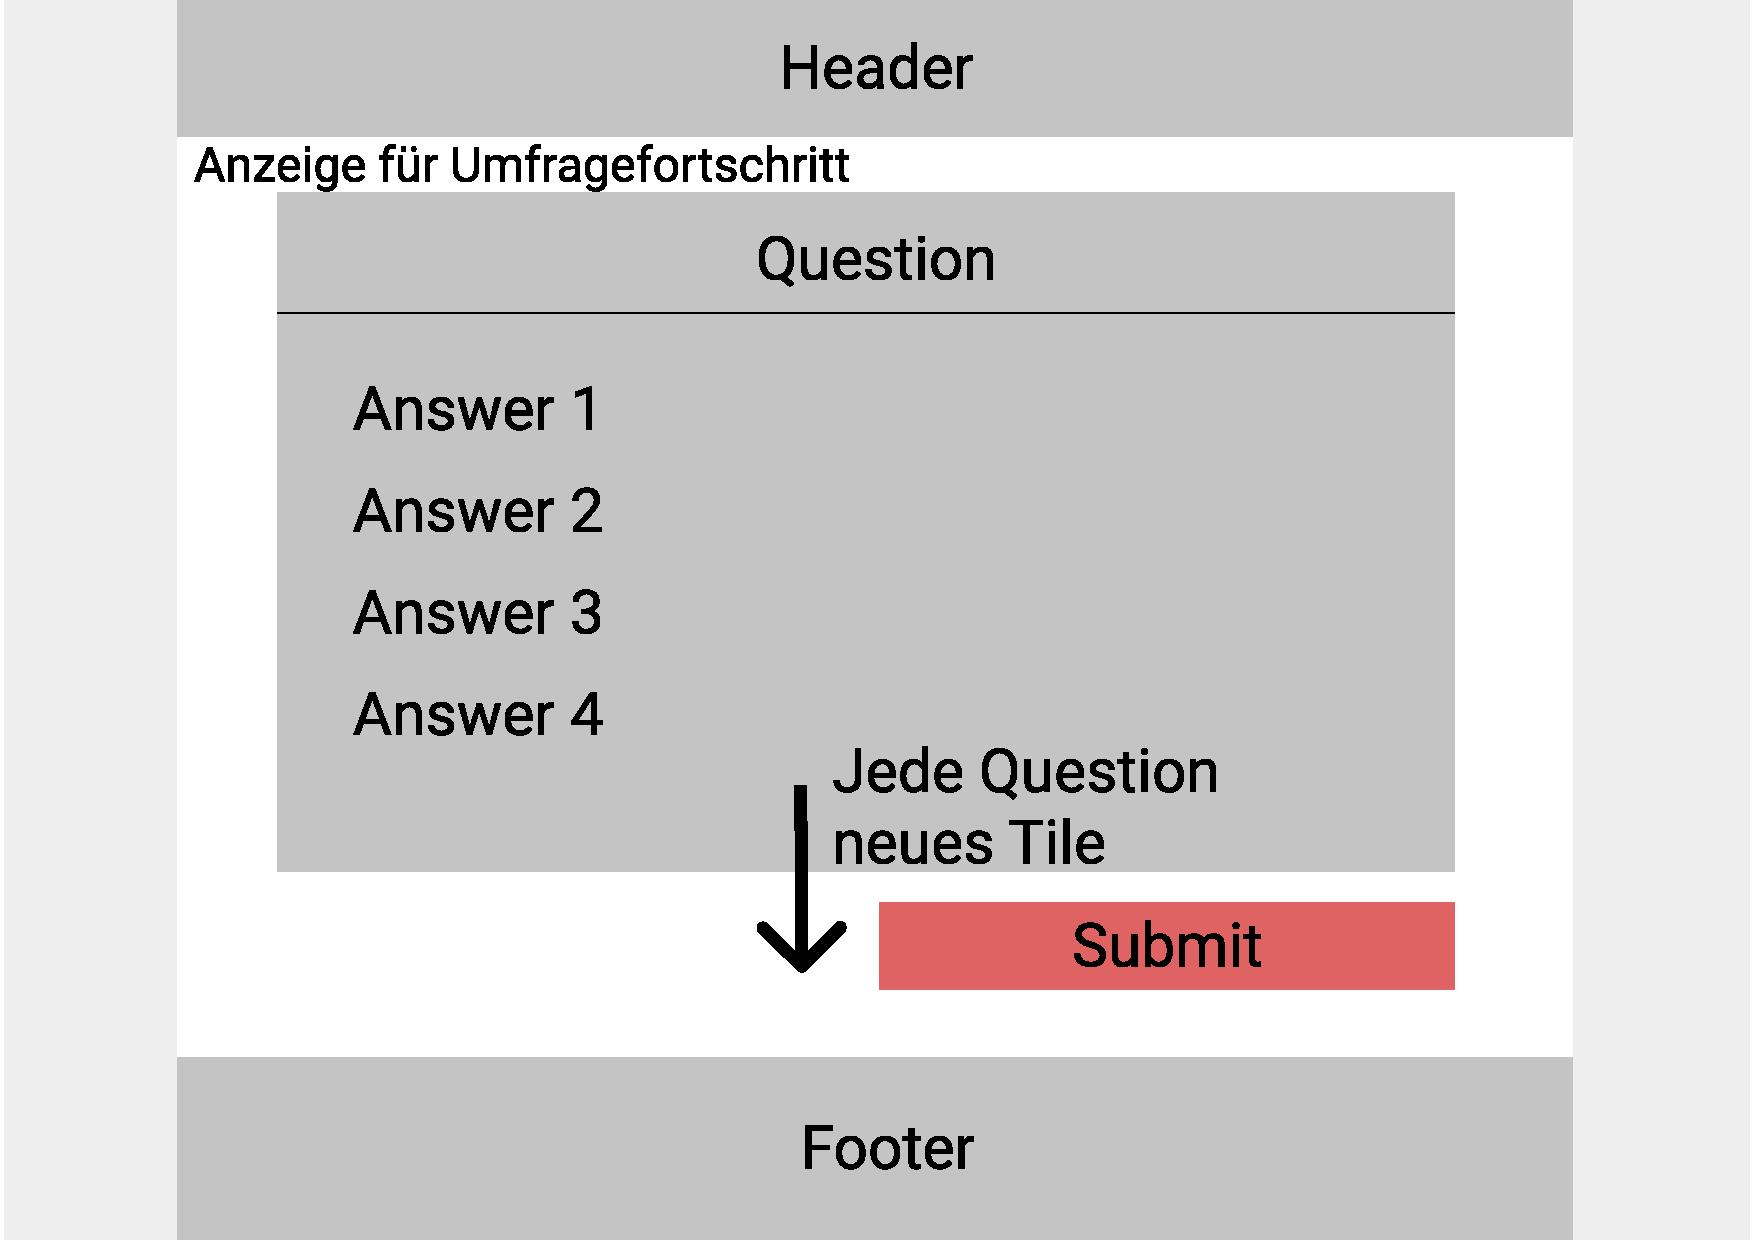
\includegraphics[width=0.7\textwidth]{img/konzeption/client/umfrage_teilnehmer}
	\captionsetup{justification=centering, format=plain}
	\caption[Mock-Up der Teilnahmeseite]{Mock-Up der Teilnahmeseite\\\figma}
	\label{fig:MockUmfrageTeilnehmer}
\end{figure}


\subsection{Result-Dashboard}
\label{ssec:ResultDashboard}





\subsection{Unterteilung der Gliederungsansichten}

\begin{itemize}
	\item Beschreibung der Mockups 
	 \begin{itemize}
		 \item Was haben wir uns bei den einzelnen Seiten gedacht
		 \item Wie sollten die Seiten grundsätzlich aussehen. (Brainstorming)
		 \item evtl. bissel auf Designthinking eingehen
		 \item Welches tool haben wir dazu genutzt
	 \end{itemize}
	 \item Recherche zu vorhandenen Umfragetools --> (https://www.polly.ai/slack-poll, https://strawpoll.de/, https://www.limesurvey.org/de/, https://www.surveymonkey.de/, https://pingo.coactum.de/)
	 --> Ideensammlung und Marktrecherche
	 \item Grundlegende Idee der Einfachheit (evtl Gesamtkonzept)
	 \item Man könnte auf den User Journey eingehen
	 \item Anlehnung an DHBW farben sind vorgesehen
	 \item Orientierung an modernen Websites mit header und footer
	 \item Hinblick auf mobile usage
\end{itemize}
\subsection{Bestimmung von Darstellungsformen}